% !TEX root = flow_head.tex
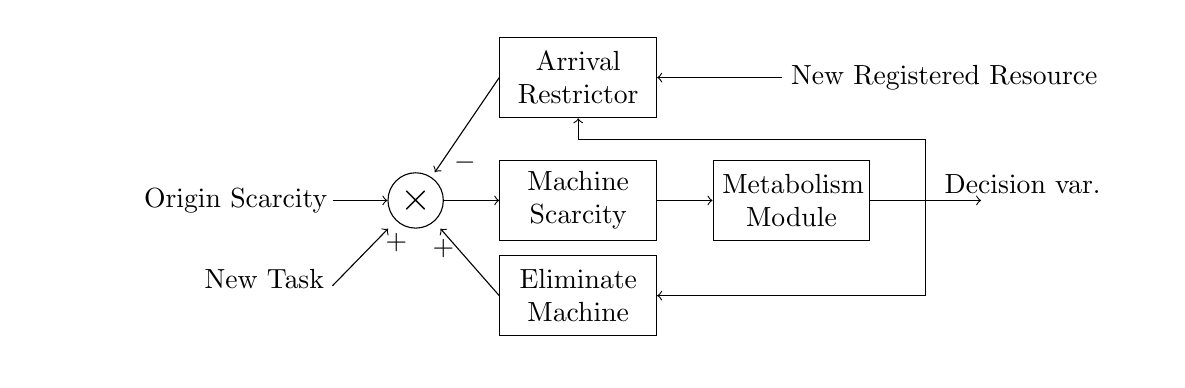
\begin{tikzpicture}[node distance=5mm and 5mm,
square/.style={
% The shape:
rectangle,
draw=black,
minimum size=2.9em,
text width=5em,
text centered
},
coord/.style={
coordinate,
% on chain,
% on grid,
% node distance=6mm and 25mm
},
circle/.style={
rectangle,minimum size=2em,rounded corners=1em,
draw=black
},
skip loop/.style={to path={-- ++(0,#1) -| (\tikztotarget)}}
]
\matrix[row sep=0.5em,column sep=2em] {
% First row:
&&&&& & & \node (machinein) [square] {Arrival Restrictor}; & \node (add) {};  &  & &\\
&&&&&&&&&&&\\
&&&&&&&&&&&\\
& & && &\node (origin2) {};  & \node (compare2) [circle] {\Large$\times$}; &  \node (scarcity) [square] {Machine Scarcity}; & \node (metabolism) [square] {Metabolism Module}; &\node (node2) [coord] {}; &\node (end2) [coord] {};\\
&&&&&\node (task) {}; &  & \node (reduce) [square] {Eliminate Machine}; &  & & &\\
&&&&& &  &  & & & & &&  \\
};
\path (add) edge[->] (machinein) (machinein.west) edge[->] (compare2) (compare2) edge[->] (scarcity) (scarcity) edge[->] (metabolism);
\path (origin2) edge[->] (compare2);
% \path (tf) edge[->] (compare2);
\path (reduce.west)  edge[->] (compare2);
\draw [->] (metabolism) -- (end2) ;
\draw [->]  (task) -- (compare2);
\path (node2) edge[->,skip loop=2.2em] (machinein);
\draw [->] (node2) |- (reduce);
\path (machinein.west) to node [near end,yshift=-0.5em,xshift=0.5em] {$-$} (compare2);
% \path (tf) to node [near end,xshift=0.5em] {$-$} (compare2);
\path (task) to node [near end,xshift=0.8em] {$+$} (compare2);
\path (reduce) to node [near end,xshift=-0.6em,yshift=-0.8em] {$+$} (compare2);
\path (node2) to node [near end,xshift=2em,yshift=0.6em] {Decision var.} (end2);
\path (add) to node [near start, xshift=7em] {New Registered Resource}(machinein) (origin2) to node [near start,xshift=-4em]{Origin Scarcity}(compare2) (task.east) to node [near start,xshift=-3em]{New Task} (compare2);
\end{tikzpicture}